\documentclass[12pt,a4paper]{amsart}
% for packages that output in tikz:
\usepackage{tikz}
% contains listings-package-related stuff incl Macaulay2 language definition:
\input lst-Macaulay2.tex
% additional options to modify appearance of code:
\lstset{
numbers=none,
frame=leftline,% comment out if you don't like the blue rectangles
framerule=1ex,
framesep=1ex,
xleftmargin=2ex,
columns=fixed,
showstringspaces=false,
breaklines=false,
}
\title{Example file for MergeTeX}
\author{Paul Zinn-Justin}
\begin{document}
\maketitle

\section{Introduction}
some basic examples:
\begin{lstlisting}[language=Macaulay2output]
`\underline{\tt i1}` : R=QQ[x,y]; factor(x^3-y^3)
`\underline{\tt o2}` = `$\left(x-y\right)\left(x^{2}+x\,y+y^{2}\right)$`
`\underline{\tt o2}` : `$\texttt{Expression}$ of class $\texttt{Product}$`
`\underline{\tt i3}` : res coker vars R
`\underline{\tt o3}` = `$\underset{\vphantom{\Big|}0}{R^{1}}\,\xleftarrow{\left(\begin{smallmatrix}
x&y
\end{smallmatrix}\right)}\,\underset{\vphantom{\Big|}1}{R^{2}}\,\xleftarrow{\left(\begin{smallmatrix}
-y\\
x
\end{smallmatrix}\right)}\,\underset{\vphantom{\Big|}2}{R^{1}}\,\xleftarrow{0}\,\underset{\vphantom{\Big|}3}{0}$`
`\underline{\tt o3}` : `$\texttt{ChainComplex}$`
`\underline{\tt i4}` : OO_(Proj(R/(x^3-y^3)))^{1,2}
`\underline{\tt o4}` = `${\mathcal O}_{\texttt{Proj}\left(\frac{R}{x^{3}-y^{3}}\right)}^{1}\left(1\right)\ \oplus \ {\mathcal O}_{\texttt{Proj}\left(\frac{R}{x^{3}-y^{3}}\right)}^{1}\left(2\right)$`
`\underline{\tt o4}` : `coherent sheaf on $\texttt{Proj}\left(\frac{R}{x^{3}-y^{3}}\right)$, free`
`\underline{\tt i5}` : matrix {{1,2},{3,4}}
`\underline{\tt o5}` = `$\left(\!\begin{array}{cc}
1&2\\
3&4
\end{array}\!\right)$`
`\underline{\tt o5}` : `$\texttt{Matrix}$ ${\mathbb Z}^{2}\,\longleftarrow \,{\mathbb Z}^{2}$`
\end{lstlisting}

The code can also be inline: \lstinline[language=Macaulay2]!gcd(1300,75)!.
More:
\begin{lstlisting}[language=Macaulay2output]
`\underline{\tt i6}` : 318/46
`\underline{\tt o6}` = `$\frac{159}{23}$`
`\underline{\tt o6}` : `${\mathbb Q}$`
`\underline{\tt i7}` : exp 3.73767
`\underline{\tt o7}` = `${42.0000160321016}$`
`\underline{\tt o7}` : `${\mathbb R}$ (of precision $53$)`
\end{lstlisting}
strings and nets:
\begin{lstlisting}[language=Macaulay2output]
`\underline{\tt i8}` : "hehe"
`\underline{\tt o8}` = `\ttfamily hehe`
`\underline{\tt i9}` : ( "haha123456789"
     ||"hoho!@#$%^&*(")
`\underline{\tt o9}` = `\ttfamily \begin{tabular}[t]{l}haha123456789\\
hoho!@{\char 35}{\char 36}{\char 37}{\char 94}{\char 38}*(\end{tabular}`
`\underline{\tt i10}` : {oo,ooo}
`\underline{\tt o10}` = `$\left\{\begin{array}{l}\texttt{haha123456789}\\
\texttt{hoho!@{\char 35}{\char 36}{\char 37}{\char 94}{\char 38}*(}\end{array},\:\texttt{hehe}\right\}$`
`\underline{\tt o10}` : `$\texttt{List}$`
\end{lstlisting}
printing:
\begin{lstlisting}[language=Macaulay2output]
`\underline{\tt i11}` : for i from 1 to 8 do print((i+ii)^2)
`${2}\,\mathbf{i}$`
`${3}+{4}\,\mathbf{i}$`
`${8}+{6}\,\mathbf{i}$`
`${15}+{8}\,\mathbf{i}$`
`${24}+{10}\,\mathbf{i}$`
`${35}+{12}\,\mathbf{i}$`
`${48}+{14}\,\mathbf{i}$`
`${63}+{16}\,\mathbf{i}$`
\end{lstlisting}

\section{Reusing output}
The output {\tt o5} is $\left(\!\begin{array}{cc}
1&2\\
3&4
\end{array}\!\right)$%\macoutput{5}
.
The nonexistent output {\tt o11} is %\macoutput{11}
.

\section{Inputting from external file}
Some more code:
\begin{lstlisting}[language=Macaulay2output]
`\underline{\tt i12}` : -- a test file
      R=QQ[x,y,z]
`\underline{\tt o12}` = `$R$`
`\underline{\tt o12}` : `$\texttt{PolynomialRing}$`
`\underline{\tt i13}` : poincare ideal(x^2+y^2,x^3+z^3)
`\underline{\tt o13}` = `$1-T^{2}-T^{3}+T^{5}$`
`\underline{\tt o13}` : `${\mathbb Z}\mathopen{}\left[T\right]$`
\end{lstlisting}

\section{Packages}
packages that have a {\tt tex} output will work:
\begin{lstlisting}[language=Macaulay2output]
`\underline{\tt i14}` : needsPackage "Posets";
`\underline{\tt i15}` : booleanLattice 3
`\underline{\tt o15}` = `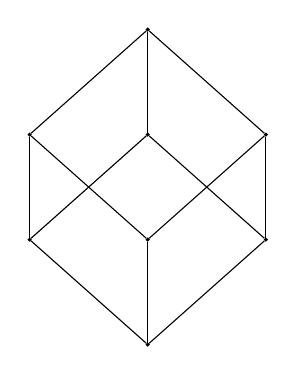
\begin{tikzpicture}[scale=1, vertices/.style={draw, fill=black, circle, inner sep=0pt}]
	\node [vertices] (0) at (-0+0,0){};
	\node [vertices] (1) at (-1.5+0,1.33333){};
	\node [vertices] (2) at (-1.5+1.5,1.33333){};
	\node [vertices] (4) at (-1.5+3,1.33333){};
	\node [vertices] (3) at (-1.5+0,2.66667){};
	\node [vertices] (5) at (-1.5+1.5,2.66667){};
	\node [vertices] (6) at (-1.5+3,2.66667){};
	\node [vertices] (7) at (-0+0,4){};
\foreach \to/\from in {0/1, 2/3, 0/2, 1/3, 4/5, 6/7, 4/6, 5/7, 0/4, 1/5, 2/6, 3/7}
\draw [-] (\to)--(\from);
\end{tikzpicture}
`
`\underline{\tt o15}` : `$\texttt{Poset}$`
`\underline{\tt i16}` : needsPackage "VectorGraphics";
`\underline{\tt i17}` : Circle{"fill"=>"red"}
`\underline{\tt o17}` = `
\begin{tikzpicture}[execute at begin picture={\bgroup\tikzset{every path/.style={}}\clip (-62,-62) rectangle ++(124,124);\egroup},x={(.0422460301541849cm,0cm)},y={(0cm,-.0422460301541849cm)},baseline=(current  bounding  box.center),every path/.style={draw=black,fill=none},line join=round]
\path[fill=red] (0,0) circle[radius=50];
\end{tikzpicture}`
`\underline{\tt o17}` : `$\texttt{Circle}$`
\end{lstlisting}

\section{Changing key/values}
\begin{lstlisting}[showstringspaces=true,language=Macaulay2output,basewidth={1.5ex}]
`\underline{\tt i18}` : "some weird spacing  and string style"
`\underline{\tt o18}` = `\ttfamily some weird spacing  and string style`
\end{lstlisting}

\section{Help}
\begin{lstlisting}[language=Macaulay2output]
`\underline{\tt i19}` : help cohomology
`\underline{\tt o19}` = `
\par \medskip\noindent\begingroup\Large\bf
cohomology -- general cohomology functor\endgroup
\par \smallskip%

\par \medskip\noindent\begingroup\Large\bf
Synopsis\endgroup
\par \smallskip%
\begin{itemize}
\item \begingroup\tt Optional\ inputs\endgroup{}:\begin{itemize}
\item \begingroup\tt Degree\endgroup{}\begingroup\tt \ ={\char 62}\ \endgroup{}\begingroup\tt ...\endgroup{}, default value 0, 
\end{itemize}

\end{itemize}

\par \medskip\noindent\begingroup\Large\bf
Description\endgroup
\par \smallskip%
\begingroup\tt cohomology\endgroup{} -- a method name available for computing expressions of the forms \begingroup\tt HH{\char 94}i(X)\endgroup{} and \begingroup\tt HH{\char 94}i(M,N)\endgroup{}.
\par If it is intended that \begingroup\tt i\endgroup{} be of class \begingroup\tt ZZ\endgroup{}, \begingroup\tt M\endgroup{} be of class \begingroup\tt A\endgroup{}, and \begingroup\tt N\endgroup{} be of class \begingroup\tt B\endgroup{}, then the method can be installed with \begingroup\tt 
\penalty-200
\vskip 4.75pt
\ \ \ \ \ cohomology(ZZ,\ A,\ B)\ :=\ opts\ -{\char 62}\ (i,M,N)\ -{\char 62}\ ...\leavevmode\hss\endgraf
\endgroup{}\vskip 4.75pt
\penalty-200\par{}

\par \medskip\noindent\begingroup\Large\bf
See also\endgroup
\par \smallskip%
\begin{itemize}
\item \begingroup\tt homology\endgroup{} -- general homology functor
\item \begingroup\tt HH\endgroup{} -- general homology and cohomology functor
\item \begingroup\tt ScriptedFunctor\endgroup{} -- the class of all scripted functors
\end{itemize}

\par \medskip\noindent\begingroup\Large\bf
Ways to use \begingroup\tt cohomology\endgroup{} :\endgroup
\par \smallskip%
\begin{itemize}
\item \begingroup\tt HH{\char 94}ZZ\ ChainComplex\endgroup{} -- cohomology of a chain complex
\item \begingroup\tt HH{\char 94}ZZ\ ChainComplexMap\endgroup{} -- cohomology of a chain complex map
\item \begingroup\tt HH{\char 94}ZZ\ Module\endgroup{} -- local cohomology of a module
\item \begingroup\tt HH{\char 94}ZZ\ SheafOfRings\endgroup{} -- cohomology of a sheaf of rings on a projective variety
\item \begingroup\tt HH{\char 94}ZZ\ SimplicialMap\endgroup{} -- Compute the induced map on cohomology of a simplicial map.
\item \begingroup\tt HH{\char 94}ZZ\ SumOfTwists\endgroup{} -- coherent sheaf cohomology module
\item \begingroup\tt {\char 34}HH{\char 94}ZZ\ CoherentSheaf{\char 34}\endgroup{} -- see \begingroup\tt HH{\char 94}ZZ(ProjectiveVariety,CoherentSheaf)\endgroup{} -- cohomology of a coherent sheaf on a projective variety
\item \begingroup\tt HH{\char 94}ZZ(ProjectiveVariety,CoherentSheaf)\endgroup{} -- cohomology of a coherent sheaf on a projective variety
\item \begingroup\tt {\char 34}HH{\char 94}ZZ\ SimplicialComplex{\char 34}\endgroup{} -- see \begingroup\tt HH{\char 94}ZZ(SimplicialComplex,Ring)\endgroup{} -- compute the reduced cohomology of an abstract simplicial complex
\item \begingroup\tt HH{\char 94}ZZ(SimplicialComplex,Ring)\endgroup{} -- compute the reduced cohomology of an abstract simplicial complex
\item \begingroup\tt HH{\char 94}ZZ(SimplicialComplex,SimplicialComplex)\endgroup{} -- compute the relative homology of two simplicial complexes
\end{itemize}

\par \medskip\noindent\begingroup\Large\bf
For the programmer\endgroup
\par \smallskip%

\par The object \begingroup\tt cohomology\endgroup{} is a \begingroup\tt method\ function\ with\ options\endgroup{}.`
`\underline{\tt o19}` : `$\texttt{DIV}$`
\end{lstlisting}

\section{Tricky examples}
\dots for testing purposes only
\begin{lstlisting}[language=Macaulay2output]
`\underline{\tt i20}` : -- some tricky examples
\end{lstlisting}
A bunch of complicated cases: a multi-line example
\begin{lstlisting}[language=Macaulay2output]
      f = i -> (
      -- that's dumb
      i+1
      )
`\underline{\tt o20}` = `$\texttt{f}$`
`\underline{\tt o20}` : `$\texttt{FunctionClosure}$`
\end{lstlisting}
and another weirder one:
\begin{lstlisting}[language=Macaulay2output]
`\underline{\tt i21}` : I=ideal 0; f = i -> (
`\underline{\tt o21}` : `$\texttt{Ideal}$ of ${\mathbb Z}$`
      i+1)
`\underline{\tt o22}` = `$\texttt{f}$`
`\underline{\tt o22}` : `$\texttt{FunctionClosure}$`
\end{lstlisting}
finally:
\begin{lstlisting}[language=Macaulay2output]
`\underline{\tt i23}` : a=1;b=2;
`\underline{\tt i25}` : c=3;
\end{lstlisting}
That last one has no output.

\end{document}
